\section{Method}\label{sec:method}

The method is a portfolio of three arms: multilevel splitting driven by transient duration (channel B), active learning of basin boundaries (channel A), and a uniform share that bounds the worst case. Prior sets (channel C) enter as a distribution of starting points and candidates. All arms receive, for each point, only its fingerprint and the label produced by the protocol of Sec.~\ref{sec:protocol}. The strategies do not know which label is the target. Two configurations are used below: the \emph{portfolio with full integration}, with which the gains in integrations of Sec.~\ref{sec:rare_ab}--\ref{sec:coupled} are measured, and the \emph{portfolio with two-stage evaluation} of Sec.~\ref{sec:twostage}, with which the costs in steps and wall time of Sec.~\ref{sec:cost} are measured.

\subsection{Reaction coordinate: transient duration}\label{sec:xi}

For an initial point $x_0$ with a trajectory fingerprint, we define
\begin{equation}
\xi(x_0)=\begin{cases}\dfrac{\ln k_{\rm esc}}{\ln N_{\rm tot}}\in[0,1], & \text{escape at step } k_{\rm esc},\\[2mm] 1+D(x_0), & \text{bounded trajectory},\end{cases}
\label{eq:xi}
\end{equation}
where
\begin{equation*}
D=\frac{\bigl\|(m_{\rm early}-m_{\rm obs},\ s_{\rm early}-s_{\rm obs})\bigr\|}{L}.
\end{equation*}
Here, $k_{\rm esc}\in\{1,\dots,N_{\rm tot}\}$ is the integration step at which the trajectory left the escape radius, $N_{\rm tot}$ is the number of integration steps, and $m$ and $s$ are the coordinate-wise means and standard deviations over the early window (the first steps of the transient segment) and over the observation window; all trajectories that escape at the first step share the value $\xi=0$. A trajectory that quickly settles onto its regime has $D\approx0$. A trajectory that lingers near an edge state on a basin boundary has a large $D$ or a large $k_{\rm esc}$. In rare-event algorithms, the levels are defined by a score (importance) function, and the optimal score is the committor, the probability of reaching the target before the alternatives.\cite{Lestang2018TAMS,Lucente2022Committor} The committor is unknown here; $\xi$ is a cheap proxy computed from a single trajectory that does not use the target label. The coordinate is built on transient rather than asymptotic features because only the former carry a signal (Appendix~\ref{app:diagnostics}): on uniform samples, transient features separate the points near the target basin from the rest with an area under the receiver operating characteristic curve (AUC) of 0.88--0.97, whereas asymptotic features (the Lyapunov exponent, the range) reach only 0.5--0.75.

\subsection{Multilevel splitting in the space of initial conditions}\label{sec:sus}

For the static problem ``initial condition $\to$ fingerprint,'' the static counterpart of adaptive multilevel splitting\cite{CerouGuyader2007} is subset simulation;\cite{AuBeck2001} below, we call it splitting. Levels are set adaptively by a quantile of $\xi$, and the sample above a level is replenished by conditional Markov chains. The algorithm is as follows.
\begin{enumerate}
\item Reference sample: $n_0=50$ uniform points of $B$.
\item The level $\xi_l$ is the value of $\xi$ at the $(n_0p_0)$th largest point, $p_0=0.2$. These $n_0p_0=10$ points are the seeds of the chains.
\item Each chain makes $1/p_0-1=4$ random-walk steps $y=x+\sigma(b-a)\eta$, $\eta\sim\mathcal{N}(0,I)$, with mirror reflection into the parallelepiped $B=[a,b]$. A step is accepted if $\xi(y)\ge\xi_l$; a rejected proposal leaves the chain in its current state, which is counted again as a state of the level. Every proposal costs one integration, so a level costs $n_0(1-p_0)=40$ integrations. For the uniform measure on $B$, a symmetric proposal with reflection, and a fixed $\sigma$, this is the Metropolis algorithm for the conditional distribution on $\{\xi\ge\xi_l\}$.
\item The step $\sigma$ (initial value 0.1) is adapted to the acceptance rate, a simple variant of adaptive proposal scaling in subset simulation:\cite{Papaioannou2015} below an acceptance rate of 0.2, it is halved; below 0.4, it is divided by 1.25; above 0.6, it is multiplied by 1.5.
\item The next level is chosen from all states of the chains of the current level (step 2). On stagnation (a relative increase of the level below 2\% or $\sigma<0.005$) for two levels, and also after 10 levels, the algorithm restarts with a new uniform reference sample.
\end{enumerate}
Restarts protect against the case in which the chains have contracted onto a nontarget region with a long transient. In the benchmark, we compared three coordinates: $\xi$ from Eq.~\eqref{eq:xi}, the escape step alone, and the multidimensional ``rarity'' of the fingerprint (the mean distance to the $k=5$ nearest neighbors in the reference sample). Figure~\ref{fig:suschains} shows how the chains of two levels are distributed over the basin map of a Jiang map, and Fig.~\ref{fig:d2mech} shows how the chains in D2 contract to the ball $|w|<\rho$.

\begin{figure}
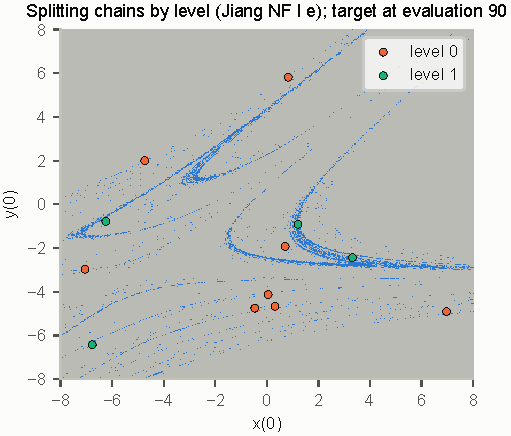
\includegraphics[width=\columnwidth]{figures/fig38_sus_chains.pdf}
\caption{Splitting chains on the basin map of the Jiang map NF~I~e (gray: escape; blue: basin of the chaotic attractor): seeds of levels 0 (open circles) and 1 (triangles). Already at the second level, the chains sit on thin ``tongues'' of the basin, since the escape step is larger near their edges; the target is found after 90 integrations. Seeds that coincide are drawn once.}
\label{fig:suschains}
\end{figure}

\subsection{Active learning of basin boundaries}\label{sec:al}

The active-learning arm stores all evaluated points with their labels; escaping trajectories form a separate class. On these data, a $k$-nearest-neighbor classifier ($k=10$, weights inversely proportional to distance) is trained in normalized coordinates of $B$. From a pool of 2000 candidates, the points with the largest entropy of the predicted class probabilities are selected for evaluation (uncertainty sampling\cite{Settles2012}). Half of the pool consists of Gaussian perturbations of ``boundary'' points of the sample, i.e., points that have a point of another class among their $k$ neighbors, with a scale of half the distance to the nearest neighbor of another class. The other half consists of uniform points or points of a prior set (nullclines). The classifier is retrained when the sample grows by 10\%. Two implementation choices keep the cost of this arm bounded (Appendix~\ref{app:implementation}): neighbors are found by brute-force search (for $n\ge6$, or while the sample has at most 2000 points), which returns the same queries several times faster than a tree, and in the two-stage configuration the classifier is trained on the last $2\times10^4$ evaluated points only. While the data contain a single class, there are no boundaries, and the arm is idle.

\subsection{Portfolio and worst-case guarantee}\label{sec:portfolio}

In each round, the portfolio evaluates a batch of points from the splitting arm (10 points), from the active-learning arm (20 points if the data contain at least two classes), and uniform points. The number of uniform points is $\lceil\theta/(1-\theta)\cdot n_{\rm arm}\rceil$, where $n_{\rm arm}$ is the number of points from the arms and $\theta=0.2$ is the uniform share. Points within a batch are shuffled so that no arm is favored in the accounting of the first-hit time. The reference sample is shared by both arms. An arm is called \emph{autonomous} if the choice of its points depends only on the results of its own evaluations. The uniform arm and the splitting arm are autonomous; the active-learning arm uses all data. The uniform share plays the role of the defensive component of mixture importance sampling,\cite{Hesterberg1995} and combining strategies with different failure modes follows the idea of algorithm portfolios, which reduce the risk of heavy-tailed run times.\cite{Huberman1997,GomesSelman2001}

\begin{proposition}\label{prop:portfolio}
Let $c$ be the maximum batch size, $\omega_j$ the guaranteed share of arm $j$ in each round, and $N_{1-\delta}(j)$ the cost of arm $j$ run on its own. Then
\begin{equation}
\begin{split}
N_{1-\delta}(\text{portfolio})\le\min\biggl\{&\frac{N^0_{1-\delta}+c}{\theta},\\
&\min_{j\ \text{autonomous}}\frac{N_{1-\delta}(j)+c}{\omega_j}\biggr\}.
\end{split}
\label{eq:portfolio}
\end{equation}
\end{proposition}
\textit{Proof.} After $N$ evaluations of the portfolio, an autonomous arm $j$ has performed at least $\omega_jN-c$ evaluations of its own. By autonomy, the sequence of its points is distributed as in a stand-alone run with the same generator. Therefore, $\Pr[\tau>N]\le\Pr[\tau_j>\omega_jN-c]\le\delta$ whenever $\omega_jN-c\ge N_{1-\delta}(j)$. For the uniform arm, $N_{1-\delta}(j)=N^0_{1-\delta}$ and $\omega_j=\theta$. \hfill$\blacksquare$

The proposition is an elementary property of a defensive mixture, and its value is in the construction it justifies. Its consequences are as follows. First, in the number of integrations, the portfolio is at most $1/\theta=5$ times costlier than uniform sampling, up to the additive term $c/\theta$: $G\ge\theta N^0/(N^0+c)$, which for $c=38$ and $N^0\approx200$ is 0.17 rather than 0.2. A single adaptive method has no such bound: splitting alone, and novelty search driven by asymptotic features (Appendix~\ref{app:ablation}), fail to find the target within the budget in some runs. Second, the scaling exponent of the portfolio is no larger than that of the best autonomous arm: a constant factor $1/\omega_j$ is lost, but not the order. In our implementation, the share of the splitting arm is $\omega\approx0.26$ when the active-learning arm is active and $\omega\approx0.77$ without it. Two qualifications apply. The bound holds in integrations, not in integrator steps or wall time: the arms select long transients, so a point of the portfolio may cost more steps than a uniform point (Sec.~\ref{sec:cost}). Autonomy of the splitting arm is exact with full integration; with two-stage evaluation and templates that grow during the search (Sec.~\ref{sec:twostage}), the coordinate of its points depends weakly on what the other arms have found, so the inheritance of its exponent is then approximate, and the bound through the uniform arm requires that stage~1 never stops a target trajectory, which is verified in Sec.~\ref{sec:cost}.

\subsection{Cost model and channel diagnostics}\label{sec:costmodel}

Splitting with selection fraction $p_0$ builds nested sets $S_l=\{\xi\ge\xi_l\}$ with $\mu(S_{l+1}\mid S_l)\approx p_0$; one level costs $n_0(1-p_0)$ evaluations. Denote by $\pi_l=\mu(W^*\mid S_l)$ the fraction of the target in the $l$th set and by $e_l=\pi_{l+1}/\pi_l\in[0,1/p_0]$ the enrichment at level $l$; $e_l<1$ means that the coordinate is deceptive at that level. The target becomes frequent when $\prod_{l<K}e_l\approx1/p$, and the cost is $N\approx n_0+n_0(1-p_0)K+O(1/\pi_K)$.

\begin{proposition}[cost model]\label{prop:cost}
Assume that the chains sample the conditional distribution on each $S_l$ exactly, that the number of levels is unbounded, and that the final stage samples $S_K$ independently. (i)~If the coordinate is ideal, $e_l=1/p_0$, then $K=\lceil\ln(1/p)/\ln(1/p_0)\rceil$ and $N=O(n_0\ln(1/p))$, i.e., $s=0$. (ii)~If the enrichment is constant, $e_l=p_0^{-\zeta}$ with $0<\zeta\le1$, then $K\approx\ln(1/p)/(\zeta\ln(1/p_0))$, and the cost is still logarithmic. (iii)~If the coordinate is informative only down to a depth $K^*$ ($e_l=1$ for $l>K^*$), then $N\approx n_0+n_0(1-p_0)K^*+1/\pi_{K^*+1}$: the scaling exponent returns to $s=1$, with a constant-factor gain $\prod_{l\le K^*}e_l$. (iv)~If the coordinate is deceptive, $e_l<1$, the same count gives a constant factor below 1, i.e., a loss.
\end{proposition}

Proposition~\ref{prop:cost} follows from counting levels. It is a model of the mechanism rather than a statement about the implementation: the implementation restarts after ten levels, so the logarithmic regime is available only while $p\ge p_0^{10\zeta}$; the states of a chain are correlated samples, which is why a coordinate with zero informative depth gives $G<1$ rather than $G=1$ (family D1, Sec.~\ref{sec:scaling_p}); and the exponent $s\approx0.45$ observed on D2 over $p=10^{-2}$--$10^{-5}$ (Sec.~\ref{sec:scaling_p}) is a crossover between the logarithmic regime at $p\gtrsim10^{-4}$ and the discretization limit below it, not an asymptotic law. Its content lies in the classification: an order-of-growth gain requires a coordinate that is informative on all scales, a finite informative depth yields a constant-factor gain, and a deceptive coordinate yields a loss. The transient duration diverges at a basin boundary, where the trajectory follows the stable manifold of the edge state. If the target basin is surrounded by such a boundary and the sets $S_l$ are nested all the way down to it, the enrichment persists on all scales (the case of D2). If the boundary of the target does not stand out against other boundaries, or if the duration saturates, only the near zone is informative. Saturation occurs, for example, for the discrete escape times of maps and for escape by slow drift.

\textbf{Diagnostics from the uniform sample.} The enrichment $e_l$ is not observable before the target is detected, but on a benchmark system with a known target, it can be estimated from a uniform sample. The decisive quantity is not the fraction of target points in the upper set $S_q$ (the fraction $q$ of points with the largest $\xi$) but spatial convergence toward the target. Let $d(q)$ be the median distance (in units of $L$) from the nontarget points of $S_q$ to the nearest target point of the sample. Splitting gains if $d(q)$ decreases as $q$ decreases: the chains move by a local random walk and need a connected ``path'' of ever longer transients leading to the basin. If $d(q)$ does not decrease, the long trajectories are scattered over the region, and there is no gain even if the fraction of the target in $S_q$ grows (Appendix~\ref{app:diagnostics}).

\textbf{Discretization limit.} The coordinate is built from a trajectory with step $\Delta t$, so escape times shorter than one step are indistinguishable. In D2, the escape time for $|w_0|\gg\rho$ equals $\rho^2/(2\kappa|w_0|^2)$, and the coordinate is informative only for $|w_0|\lesssim\rho/\sqrt{2\kappa\Delta t}$. The size of this zone relative to the region sets the limit of the gain at small $p$ and small $m$ (Sec.~\ref{sec:scaling_p}, Appendix~\ref{app:smallp}).

\subsection{Two-stage evaluation}\label{sec:twostage}

Most of the integration budget goes to trajectories that settle early onto a known regime yet are integrated over the full horizon, which the protocol requires only for target candidates (Sec.~\ref{sec:protocol}). We therefore evaluate every initial condition in two stages, for all strategies including uniform sampling. Stage~1 integrates the transient segment up to the end of the early window, $\min(n_{\rm tr},n_{\rm obs})$ steps, where $n_{\rm tr}$ and $n_{\rm obs}$ are the numbers of steps of the transient segment and of the observation window, followed by a short observation window of $n_{\rm obs}/4$ steps. The trajectory stops after stage~1 if, on this window, it is identified with confidence as a known nontarget regime: an equilibrium (converged, or decaying with an amplitude below $0.02L$), or a known cycle or chaotic attractor with a $z$ score below half the identification tolerance. Escaping trajectories are final anyway. All other trajectories (target candidates and unknown or ambiguous ones) continue from the end of the early window to the full horizon. Since the main trajectory and the early window are the same, their fingerprints coincide bit for bit with those of a single full integration, and the target is always confirmed by the full protocol. A stopped trajectory keeps its label; only its $\xi$ is computed on the shorter window.

For continued trajectories, stage~1 costs extra steps, because a quarter of the observation window is integrated twice. A rule based on step counts therefore keeps the two-stage mode only while it pays. After the first 200 evaluations, the mode stays on as long as the steps saved over the last ten batches exceed the extra steps; otherwise, only every tenth batch is evaluated in two stages, as a probe. The rule uses step counts rather than time, so runs remain reproducible. On uniform samples from eight problems, the two-stage labels and the fingerprints of all continued and escaping trajectories coincided with those of full integration bit for bit, and no target hit was lost (Sec.~\ref{sec:cost}).
